% !TeX root = ..//diffgeo_main.tex
\begin{defs}[Differenzierbare Mannigfaltigkeit]
Eine \textit{differenzierbare Struktur} auf einer topologischen Mannigfaltigkeit M ist ein \textit{maximaler $C^\infty$-Atlas}. Eine \textit{differenzierbare Mannigfaltigkeit} ist eine topologische Mannigfaltigkeit mit einer differenzierbaren Struktur.
\end{defs}

\begin{bem}
Man kann auch eine topologische Mannigfaltigkeit definieren, ohne das 2. Abzählbarkeitsaxiom zu fordern.
\begin{description}
\item[Aber:] Dann bekommt man Mannigfaltigen mit ganz anderen Eigenschaften als diejenigen, die wir betrachten wollen.
\item[Wichtig:] Hausdorffsch + 2. Abzählbarkeitsaxiom $\Rightarrow$ parakompakt, d. h. jede offene Überdeckung hat eine lokale Verfeinerung.
\end{description}
$(V_j)$ heißt Verfeinerung von $(U_j)$, falls $\forall V_j \exists U_j$ mit $V_j \subseteq U_j$\\
Lokal endlich: $\forall p \in X\ \exists$ Umgebung $U$, die nur endlich viele $U_i$ trifft\\
Parakompakt $\Rightarrow \exists$ Partition der Eins f mit 
\begin{align*}
f_i: V_i \subseteq X \rightarrow [0, 1],\ \sum_{i \in I} f_i (x) = 1
\end{align*} 
\end{bem}

\begin{bsp}
Metrische Räume sind parakompakt.
\end{bsp}

\begin{bsp}[differenzierbare Mannigfaltigkeiten]
\begin{enumerate}
\item$\mathbb{R}^n$ mit Atlas $\mathcal{A} = \{(\operatorname{id}, \R^n)\}$
\item$V$ Vektorraum, $B$ Basis mit $B = \{v_1, \cdots, v_n\}$, Atlas $\mathcal{A} = \set{(\chi_B, V)}$
\begin{align*}
& \chi_B: V \rightarrow \R^n\\
& v = \sum^n_{i=1} a_i v_i \mapsto \sum_{i=1}^n a_i e_i
\end{align*}
wobei $(e_1, \cdots, e_n)$ die Standartbasis ist.
\item$M\subseteq \R^n,\ (\chi_U, U)$ mit $\chi_U = \operatorname{id}\vert_U,\ V \subseteq M^n,\ M$ differenzierbare Mannigfaltigkeit, $\mathcal{A} = \set{(\chi_X, U)}$ Atlas von $M$\\
$\mathcal{A}_V = \set{(\chi_V, U_V}$ wobei $(\chi_V, U_V) = (\chi_{U\cap V}, U\cap V)$
\item$M_1 = S^1,\ M_2 = \R,\ M_1\times M_2 =$ "unendlicher Zylinder"
\end{enumerate}
\hspace{.06\textwidth}
\begin{minipage}[H]{0.8\textwidth}
Seien $M_1^{n_1}, M_1^{n_2}$ differenzierbare Mannigfaltigkeiten, so ist $M_1\times M_2$ ebenfalls eine \difM \ der Dimension $n_1 + n_2$.\\
Atlas $\mathcal{A} = \set{(x\times y, U\times V)}$, wobei 
\begin{align*}
(x, U) &= \text{Karte von } M_1\\
(y, V) &= \text{Karte von } M_2
\end{align*}
$(x\times y)(p_1, p_2) = (x(p_1), y(p_2))$
\end{minipage}
\hspace{1cm}
\begin{minipage}[H]{.2\textwidth}
\vspace{-1.5cm}
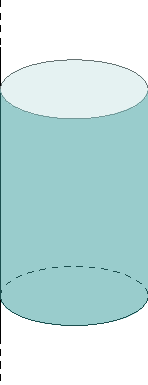
\includegraphics[scale=0.5]{figures/tikz/cylinder.pdf}
\end{minipage}
\end{bsp}

\begin{bem}
$N$ mit der Teilraumtopologie und dem Atlas $\mathcal{A}_N = \set{(\chi\vert_U, U\cap N)}$ ist eine \difM.
\end{bem}

\begin{defs}
Seien $M, N$ differenzierbare Mannigfaltigkeiten. Eine \textit{Einbettung} ist eine differenzierbare Abbildung
\begin{align*}
f: N \rightarrow M
\end{align*}
sodass
\begin{enumerate}
\item$f(N)\subset M$ eine Untermannigfaltigkeit 
\item$f: N \rightarrow f(N)$ Diffeomorphismus
\end{enumerate}
\end{defs}

\section{Tangentialraum} 

\missingfigure{Tangentialräume}

\begin{defs}
\begin{enumerate}
\item Ein Tangentialvektor an $M$ im Punkt $p \in M$ ist eine $\R$-lineare Abbildung
\begin{align*}
v: \mathcal{F}(M) \rightarrow \R
\end{align*}
mit $v(fg) = v(f)g(p) + f(p)v(g)$.
\item Die Menge aller Tangentialvektoren an $M$ in $p$ heißt \textit{Tangentialraum} von $M$ in $p$: $T_pM$\\
$T_pM$ ist ein Vektorraum.
\end{enumerate}

\begin{figure}[H]
\centering
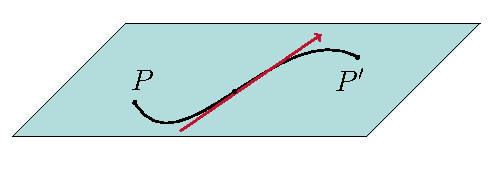
\includegraphics[scale=1]{figures/tikz/tangentline.pdf}
\end{figure}

\end{defs}
